\documentclass[14pt, a4paper]{report}
\usepackage{mathtext}
\usepackage[T2A]{fontenc}
\usepackage[utf8]{inputenc}
\usepackage[russian]{babel}
\usepackage{multirow}
\usepackage{slashbox}
\usepackage{makecell}
\usepackage{graphicx}
\usepackage{physics}
\usepackage{amstext}
\usepackage{caption}
\usepackage{subcaption}
\usepackage{cmap}
\usepackage{float}
\usepackage{indentfirst}
\usepackage{romannum}
\usepackage{wasysym}

\usepackage[a4paper,
            		left=1in,
            		right=1in,
           		 top=1in,
            		bottom=1in,
            		footskip=.25in]{geometry}

\renewcommand{\thesection}{\arabic{section}.}
\renewcommand{\thesubsection}{\arabic{section}.\arabic{subsection}.}

\title{\textbf{Объяснение аномального смещения перигелия орбиты Меркурия в рамках общей теории относительности}}
\author{Калашников Михаил, Б03-202}
\date{}

\begin{document}
\maketitle

\pagenumbering{arabic}

\section{Обнаружение эффекта}

В 1859 французский математик Урбен Жан Жозеф Леверье опубликовал работу «Новое определение орбиты Меркурия и ее возмущений», в которой предельно строго и подробно изучил движение ближайшей к Солнцу планеты. Главным результатом работы была аномальная прецессия перигелии орбиты Меркурия, которая не могла быть объяснена в рамках ньютоновой механики.

\begin{figure}[H]
\centering
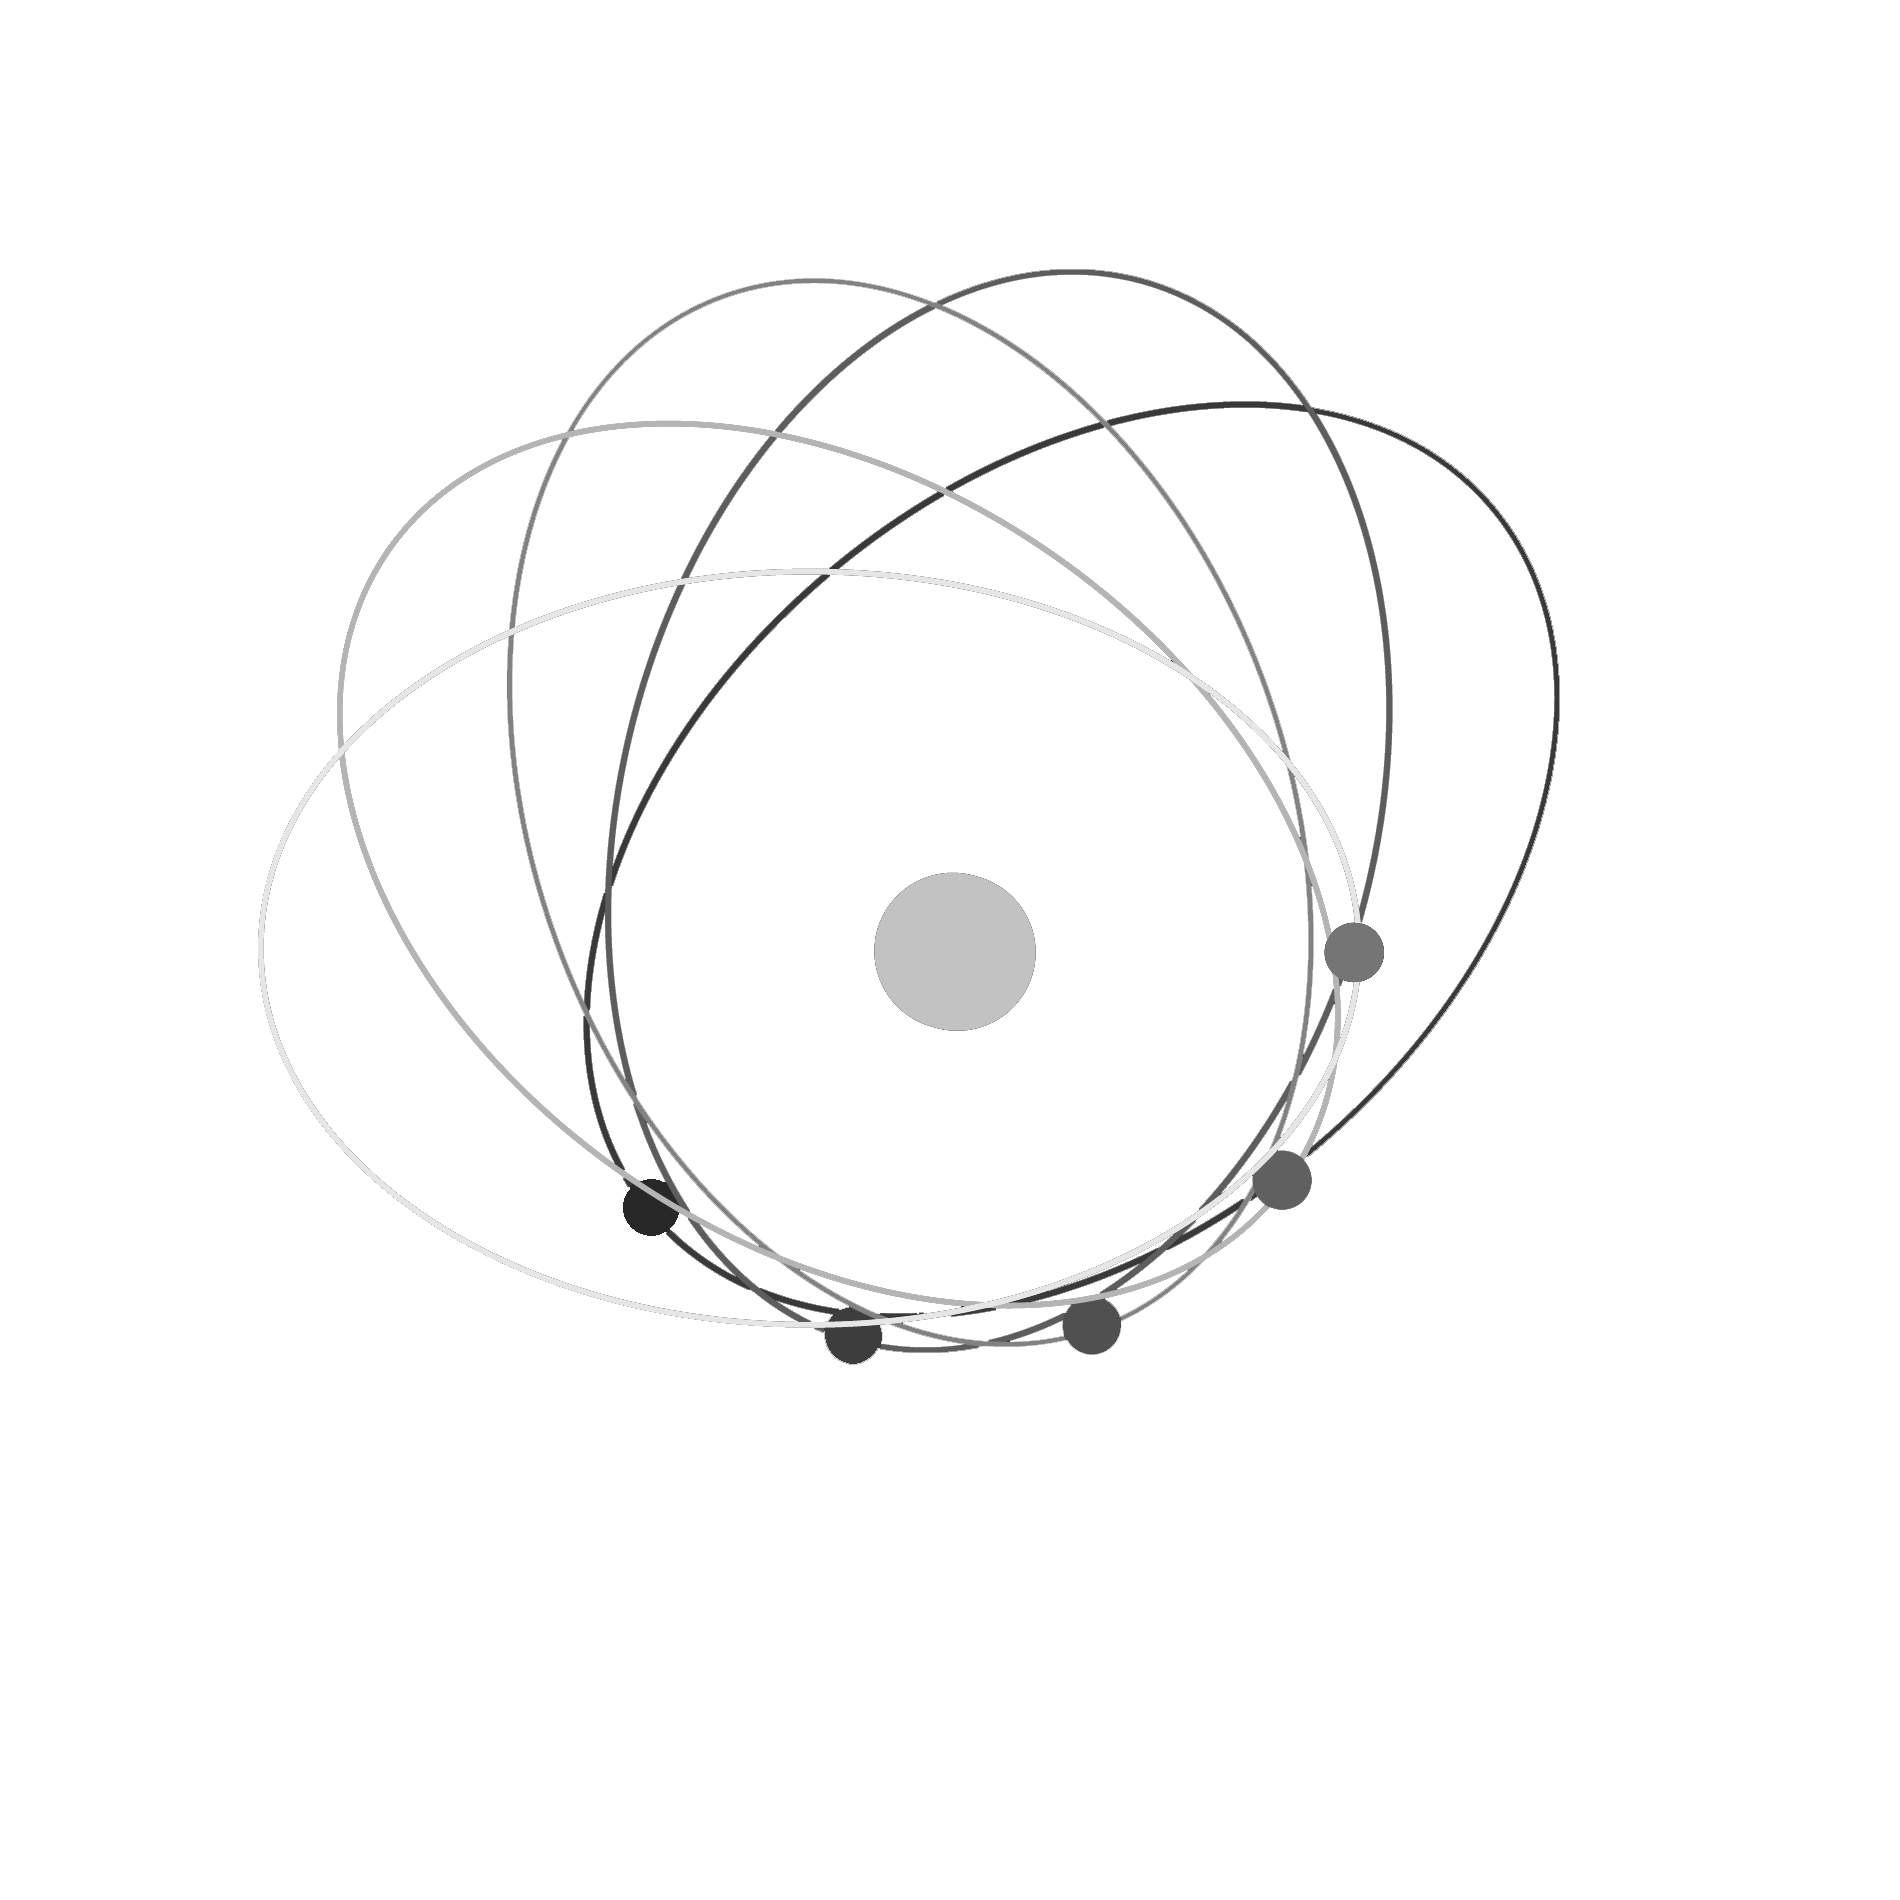
\includegraphics[width=0.6\linewidth]{../images/mc-1}
\caption{Схематичное представление прецессии линии апсид орбиты}
\end{figure}

Наблюдаемая прецессия за столетие составляла $570^{\prime\prime}$. Воздействие остальных планет Солнечной системы и несферичности Солнца могло объяснить только $526.7^{\prime\prime}$ прецессии. Таким образом, разница составила около $43^{\prime\prime}$ за столетие.

Для решения проблемы выдвигались различные теории, в основном относящиеся к одной из двух групп:
\begin{itemize}
\item гипотезы, объясняющие смещение некоторой необнаруженной материей внутри орбиты Меркурия;
\item теории гравитационного тяготения, отличающиеся от ньютоновской.
\end{itemize}

Самое элегантное и точное объяснение было найдено Альбертом Эйнштейном 18 ноября 1915 года. В рамках общей теории относительности Эйнштейн приближенно рассчитал аномальное отклонение и смог получить практически точное совпадение с наблюдаемыми $43^{\prime\prime}$ за столетие.

\section{Движение частицы в метрике Шварцшильда}

В специальной теории относительности показано, что расстояние между двумя точками пространства-времени задается метрикой
\[ds^2=c^2dt^2-dx^2-dy^2-dz^2\]
в декартовых координатах. В сферических метрика может быть записана как
\[ds^2=c^2dt^2-dr^2-r^2d\theta^2-r^2\sin^2\theta d\varphi^2\]

Эта формула справедлива в отсутствие кривизны пространства-времени. В общей теории относительности пространство времени искривлено. Согласно ей, пространство-время в гравитационном поле сферически-симметрично распределенной материи описывается метрикой Шварцшильда
\[ds^2=\left(1-\frac{r_s}{r}\right)c^2dt^2-\frac{dr^2}{1-\frac{r_s}{r}}-r^2d\theta^2-r^2\sin^2\theta d\varphi^2\]
где $r_s=\frac{2\mu}{c^2}$ -- радиус Шварцшильда, а $\mu=GM$ -- гравитационный параметр, являющийся произведением гравитационной постоянной и массы тела. При отсутствии массы $M$ метрика Шварцшильда переходит в метрику неискривленного пространства.

В соответствии с общей теорией относительности, свободные частицы пренебрежимо малой массы движутся по геодезическим линиям пространства-времени.

Ввиду сферической симметричности можно ограничится рассмотрением движения в плоскости $\theta=\frac{\pi}{2}$:
\[ds^2=\left(1-\frac{r_s}{r}\right)c^2dt^2-\frac{dr^2}{1-\frac{r_s}{r}}-r^2 d\varphi^2\]

Данный вид метрики не зависит от координат $t$ и $\varphi$. Из этого следует, что существует два интеграла движения (доказательство представлено в конце работы)
\[r^2\frac{d\varphi}{d\tau}=\frac{L}{m}\]
\[\left(1-\frac{r_s}{r}\right)\frac{dt}{d\tau}=\frac{E}{mc^2}\]
где $L$ -- момент импульса, $E$ -- полная энергия пробного тела массой $m$.

Поделим метрику на квадрат дифференциала собственного времени $d\tau^2$, учитывая, что $ds\equiv cd\tau$, и подставим первые интегралы
\[c^2=\left(1-\frac{r_s}{r}\right)c^2\left(\frac{dt}{d\tau}\right)^2-\frac{1}{1-\frac{r_s}{r}}\left(\frac{dr}{d\tau}\right)^2-r^2\left(\frac{d\varphi}{d\tau}\right)^2\]
\[\left(\frac{dr}{d\tau}\right)^2=\frac{E}{m^2c^2}-\left(1-\frac{r_s}{r}\right)\left(c^2+\frac{L^2}{m^2r^2}\right)\]

Используя определение радиуса Шварцшильда, получим
\[\frac{1}{2}m\left(\frac{dr}{d\tau}\right)^2=\left[\frac{E^2}{2mc^2}-\frac{1}{2}mc^2\right]+\frac{\mu m}{r}-\frac{L^2}{2mr^2}+\frac{\mu L^2}{c^2 mr^3}\]

Это соответствует движению нерялетивистской частинцы с энергией $\frac{E^2}{2mc^2}-\frac{1}{2}mc^2$ в радиально симметричном эффективном потенциальном поле
\[U_{эфф}(r)=-\frac{\mu m}{r}+\frac{L^2}{2mr^2}-\frac{\mu L^2}{c^2 mr^3}\]

В классической механике движение в центральном поле описывается потенциалом
\[U_{эфф}(r)=-\frac{\mu m}{r}+\frac{L^2}{2mr^2}\]

Таким образом, третий член, обратно пропорциональный кубу расстояния до гравитирующего тела, не имеет аналога в классической задаче Кеплера.

Введем обозначение $a=\frac{L}{mc}$. Тогда, используя определение радиуса Шварцшильда, потенциал можно записать в безразмерном виде
\[U_{эфф}(r)=\frac{mc^2}{2}\left[-\frac{r_s}{r}+\frac{a^2}{r^2}-\frac{r_s a^2}{r^3}\right]\]

\section{Круговые орбиты и их устойчивость}

Рассмотрим круговые орбиты в рамках данного эффективного потенциала. Очевидно, что при движении по круговой орбите, эффективная радиальная сила, действующая на частицу, должна равняться нулю.
\[F=-\frac{dU_{эфф}}{dr}=-\frac{mc^2}{2r^4}\left[r_s r^2-2a^2 r+3r_s a^2\right]=0\]

Решением данного квадратного уравнения являются два радиуса
\[r_{внешн}=\frac{a^2}{r_s}\left(1+\sqrt{1-\frac{3r_s^2}{a^2}}\right)\]
\[r_{внутр}=\frac{a^2}{r_s}\left(1-\sqrt{1-\frac{3r_s^2}{a^2}}\right)=\frac{3a^2}{r_{внешн}}\]

Внутренний радиус $r_{внутр}$ является точкой максимума потенциала, и следовательно является неустойчивым положением при любых значениях параметра $a$. Внешний радиус $r_{внешн}$, наоборот, является радиусом стабильных орбит.

Условием перехода к классическому случаю является $r_s\ll a$. Это условие можно переписать в виде
\[\frac{r_s}{a}=\frac{\mu}{c^2}\frac{mc}{L}=\frac{\mu m}{Lc}\sim\frac{\mu m}{mvrc}=\frac{\mu}{vrc}\sim\frac{v^2}{vc}=\frac{v}{c}\ll 1\]

В данном приближении внешний устойчивый радиус $r_{внешн}$
\[r_{внешн}\approx\frac{a^2}{r_s}\left(1+\left(1-\frac{3r_s^2}{2a^2}\right)\right)=\frac{a^2}{r_s}\left(2-\frac{3r_s^2}{2a^2}\right)\approx\frac{2a^2}{r_s}\]

Подставляя определения $a$ и $r_s$ можно получить классическую формулу для радиуса круговой орбиты. 
\[r_{внешн}\approx\frac{L^2}{\mu m^2}=\frac{v^2 r_{внешн}^2}{\mu}=\frac{\omega_\varphi^2 r_{внешн}^4}{\mu}\]
\[r_{внешн}^3\approx\frac{\mu}{\omega_\varphi^2}\]

\begin{figure}[H]
\centering
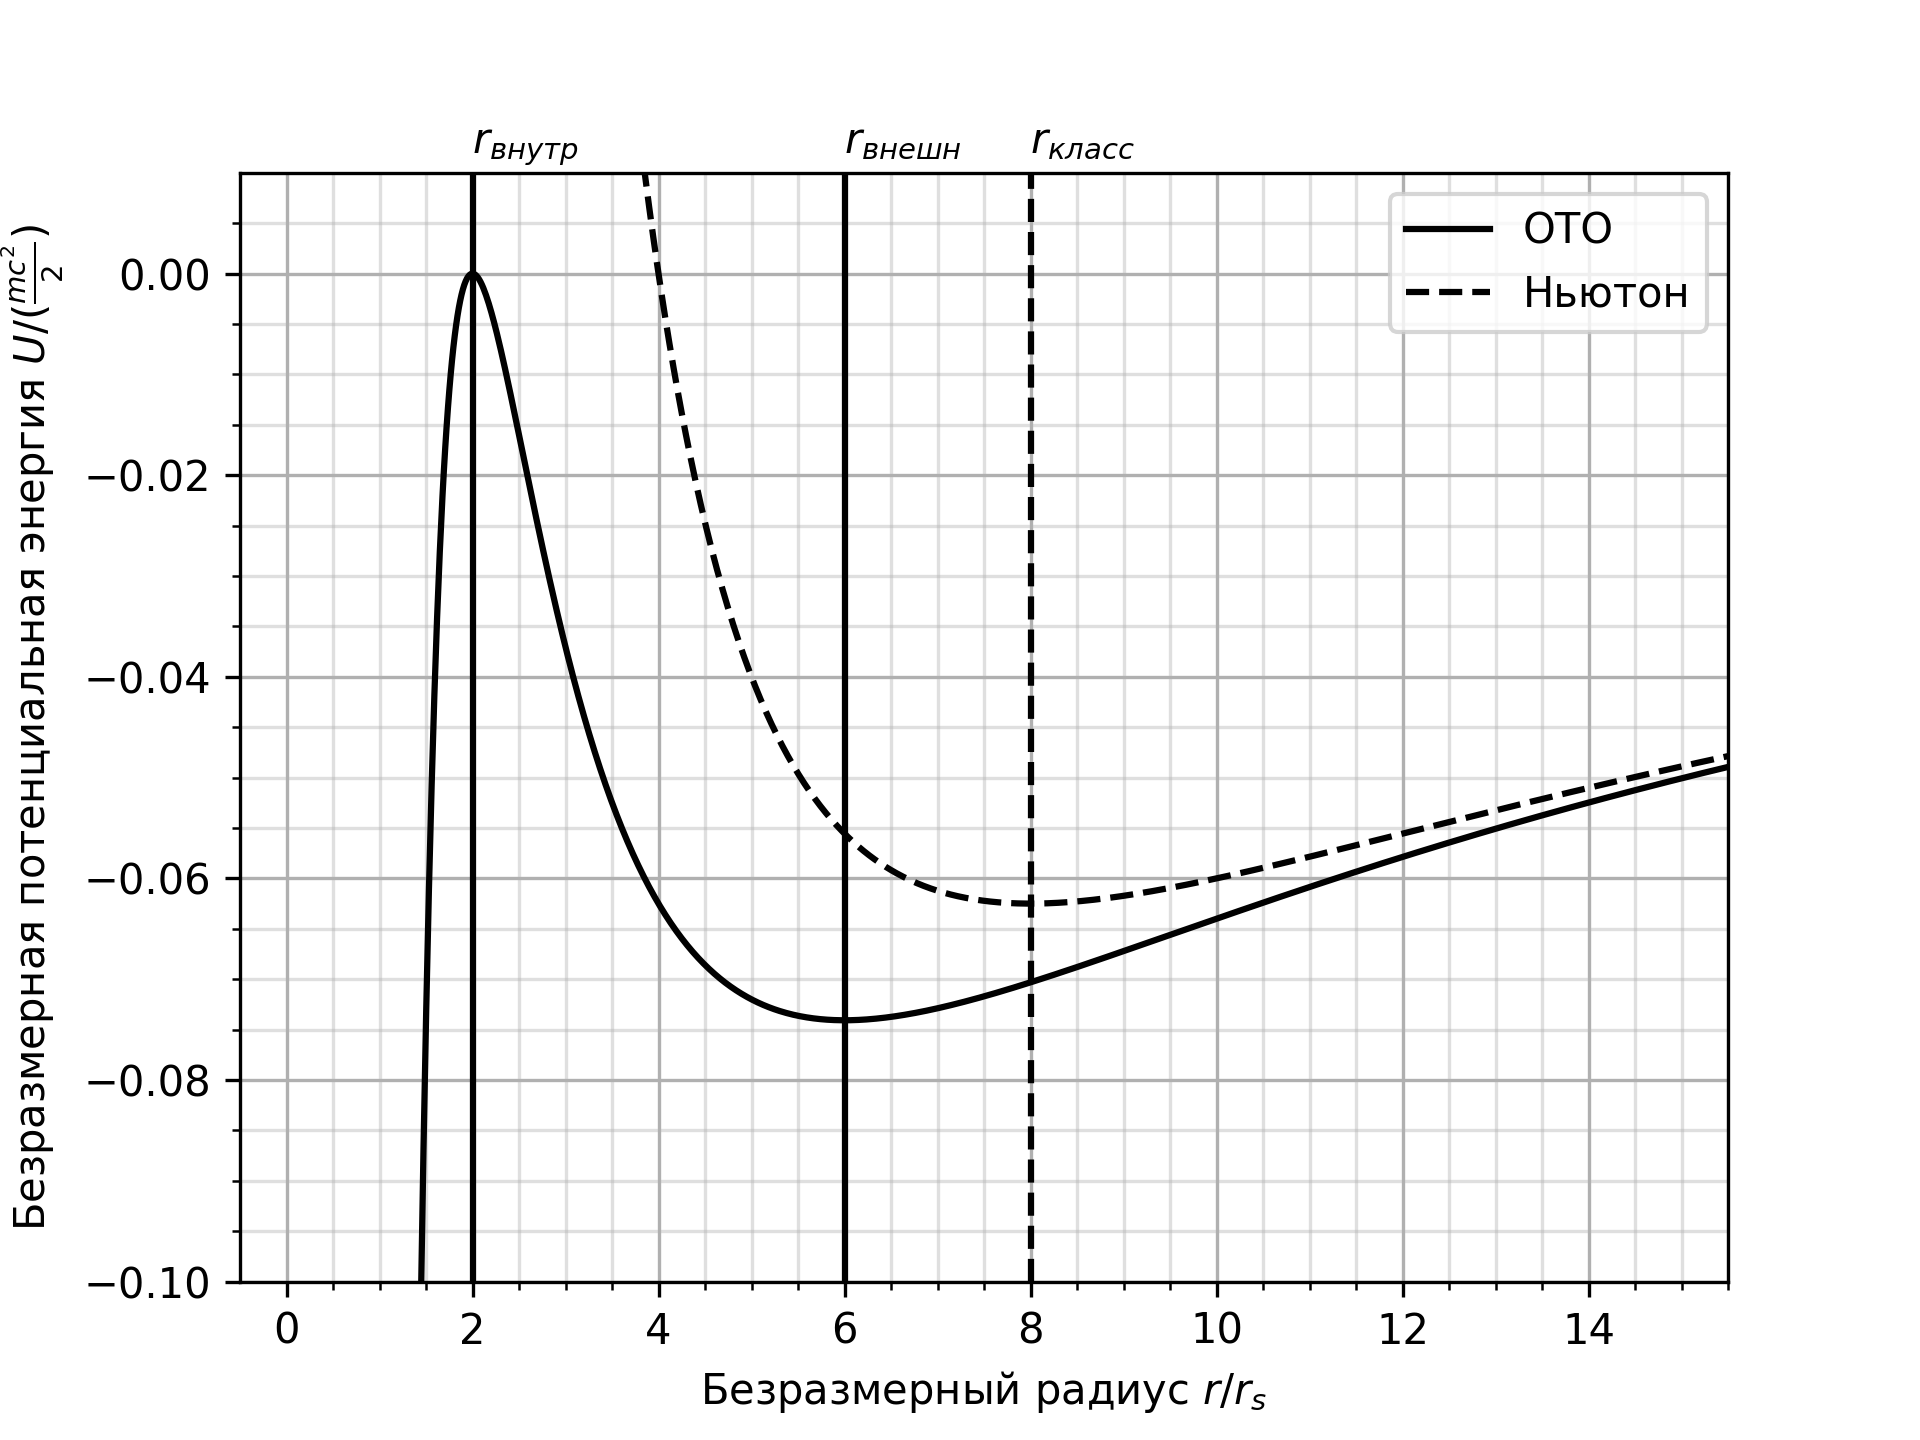
\includegraphics[width=0.7\linewidth]{../images/mc-2}
\caption{Сравнение эффективных потенциалов. $a/r_s=2$}
\end{figure}

На графике выше представлены зависимости потенциальной энергии в обеих теориях. 
\[\left(\frac{U_{эфф}(r/r_s)}{\frac{mc^2}{2}}\right)_{ОТО}=-\frac{1}{r/r_s}+\frac{a^2}{r_s^2}\frac{1}{(r/r_s)^2}-\frac{a^2}{r_s^2}\frac{1}{(r/r_s)^3}\]
\[\left(\frac{U_{эфф}(r/r_s)}{\frac{mc^2}{2}}\right)_{класс}=-\frac{1}{r/r_s}+\frac{a^2}{r_s^2}\frac{1}{(r/r_s)^2}\]

Можно отметить, что при $r/r_s\gg 1$ функции совпадают. При переходе к классическому приближению графики так же начинают сливаться, а $r_{внешн}$ переходит в $r_{класс}$.

\section{Прецессия эллиптических орбит}

Рассмотрим малое отклонение вдоль радиуса от устойчивой круговой орбиты.
Возвращающая сила будет равна
\[F(r+\Delta r)|_{r_{внешн}}\approx\frac{dF}{dr}|_{r_{внешн}}\Delta r=-\frac{d^2 U_{эфф}}{dr^2}|_{r_{внешн}}\Delta r\]

Тогда гармонические колебания около положения равновесия $r_{внешн}$ будут происходить с угловой частотой
\[\omega_r^2=\frac{1}{m}\frac{d^2 U_{эфф}}{dr^2}|_{r_{внешн}}=\frac{a^2 c^2}{r_{внешн}^4}\sqrt{1-\frac{3r_s^2}{a^2}}\approx\omega_\varphi^2\sqrt{1-\frac{3r_s^2}{a^2}}\]
\[\omega_r\approx\omega_\varphi\sqrt[4]{1-\frac{3r_s^2}{a^2}}\approx\omega_\varphi\left(1-\frac{3r_s^2}{4a^2}\right)\]

Разность данных угловых скоростей будет соответствовать скорости поворота линии апсид эллиптической орбиты. За один «период» линия апсид орбита повернется на угол
\[\delta\varphi=T(\omega_\varphi-\omega_r)\approx T\omega_\varphi\left(1-1+\frac{3r_s^2}{4a^2}\right)=2\pi\frac{3r_s^2}{4a^2}=\frac{6\pi\mu^2 m^2}{c^2 L^2}\]

Из классической небесной механики известно, что
\[\frac{L}{m}=\sqrt{\mu p}\]
где $p$ -- фокальный параметр эллипса. Он может быть выражен через кеплеровы элементы как $p=A(1-e^2)$. Здесь $A$ -- большая полуось, $e$ -- эксцентриситет. Подставим данное соотношение в $\delta\varphi$.
\[\delta\varphi\approx\frac{6\pi\mu}{c^2 A(1-e^2)}\]

Данное выражение является наиболее известной приближенной формулой прецессии. Подставляя параметры орбиты Меркурия, получим $\delta\varphi_{\mercury}\approx0.1035^{\prime\prime}$. За столетие эта величина составляет недостающие $42.98^{\prime\prime}$.

\section{Вывод}

Общая теория относительности Эйнштейна полностью объяснила расхождения в движении Меркурия, обнаруженные Леверье. А сама задача явилась одним из многочисленных подтверждений ОТО. Позже были измерены аномальные прецессии перицентров орбит остальных планет солнечной системы, некоторых астероидов и даже тесных двойных звездных систем. Значения для различных тел варьируются от сотых долей угловой секунды до десятков градусов в год, но все с высокой точностью подтверждаются теорией Эйнштейна.

\newpage

\section{Доказательство существования первых интегралов}

Как упоминалось ранее, согласно общей теории относительности свободные частицы с пренебрежимо малой массой движутся по геодезическим линиям в пространстве-времени. Последние определяются как кривые, малые вариации которых не изменяют их длину. Это можно записать как
\[0=\delta s=\delta\int ds=\delta\int\sqrt{\left(\frac{ds}{d\tau}\right)^2}d\tau\]

Производная $\frac{ds}{d\tau}$ была выражена ранее. Её квадрат может быть представлен как
\[\left(\frac{ds}{d\tau}\right)^2=c^2=\left(1-\frac{r_s}{r}\right)c^2\left(\frac{dt}{d\tau}\right)^2-\frac{1}{1-\frac{r_s}{r}}\left(\frac{dr}{d\tau}\right)^2-r^2\left(\frac{d\varphi}{d\tau}\right)^2\]

Занесем вариацию под интеграл
\[0=\delta\int\sqrt{\left(\frac{ds}{d\tau}\right)^2}d\tau=\int\frac{\delta\left(\frac{ds}{d\tau}\right)^2}{2\sqrt{\left(\frac{ds}{d\tau}\right)^2}}d\tau=\int\frac{\delta\left(\frac{ds}{d\tau}\right)^2}{2c}d\tau=\frac{1}{2c}\delta\int\left(\frac{ds}{d\tau}\right)^2 d\tau\]

Решение вариационной задачи задаётся уравнениями Лагранжа
\[\frac{d}{d\tau}\left(\frac{\partial \left(\frac{ds}{d\tau}\right)^2}{\partial \left(\frac{dx_i}{d\tau}\right)}\right)=\frac{\partial \left(\frac{ds}{d\tau}\right)^2}{\partial x_i}\]

Применим уравнение Лагранжа к координатам $t$ и $\varphi$
\[\frac{d}{d\tau}\left[2c^2\left(1-\frac{r_s}{r}\right)\frac{dt}{d\tau}\right]=0\]
\[\frac{d}{d\tau}\left[2r^2\frac{d\varphi}{d\tau}\right]=0\]

Следовательно, следующие величины являются интегралами движения
\[\frac{E}{mc^2}=\left(1-\frac{r_s}{r}\right)\frac{dt}{d\tau}\]
\[\frac{L}{m}=r^2\frac{d\varphi}{d\tau}\]

Переход к классическому приближению позволяет показать, что данные первые интегралы в дейстивтельности являются энергией и моментом импульса пробного тела.

\end{document}